\documentclass[]{article}
\usepackage{lmodern}
\usepackage{amssymb,amsmath}
\usepackage{ifxetex,ifluatex}
\usepackage{fixltx2e} % provides \textsubscript
\ifnum 0\ifxetex 1\fi\ifluatex 1\fi=0 % if pdftex
  \usepackage[T1]{fontenc}
  \usepackage[utf8]{inputenc}
\else % if luatex or xelatex
  \ifxetex
    \usepackage{mathspec}
  \else
    \usepackage{fontspec}
  \fi
  \defaultfontfeatures{Ligatures=TeX,Scale=MatchLowercase}
\fi
% use upquote if available, for straight quotes in verbatim environments
\IfFileExists{upquote.sty}{\usepackage{upquote}}{}
% use microtype if available
\IfFileExists{microtype.sty}{%
\usepackage{microtype}
\UseMicrotypeSet[protrusion]{basicmath} % disable protrusion for tt fonts
}{}
\usepackage[margin=1in]{geometry}
\usepackage{hyperref}
\hypersetup{unicode=true,
            pdftitle={rmarkdown\_pdf},
            pdfauthor={Sébastien Renaut},
            pdfborder={0 0 0},
            breaklinks=true}
\urlstyle{same}  % don't use monospace font for urls
\usepackage{color}
\usepackage{fancyvrb}
\newcommand{\VerbBar}{|}
\newcommand{\VERB}{\Verb[commandchars=\\\{\}]}
\DefineVerbatimEnvironment{Highlighting}{Verbatim}{commandchars=\\\{\}}
% Add ',fontsize=\small' for more characters per line
\usepackage{framed}
\definecolor{shadecolor}{RGB}{248,248,248}
\newenvironment{Shaded}{\begin{snugshade}}{\end{snugshade}}
\newcommand{\AlertTok}[1]{\textcolor[rgb]{0.94,0.16,0.16}{#1}}
\newcommand{\AnnotationTok}[1]{\textcolor[rgb]{0.56,0.35,0.01}{\textbf{\textit{#1}}}}
\newcommand{\AttributeTok}[1]{\textcolor[rgb]{0.77,0.63,0.00}{#1}}
\newcommand{\BaseNTok}[1]{\textcolor[rgb]{0.00,0.00,0.81}{#1}}
\newcommand{\BuiltInTok}[1]{#1}
\newcommand{\CharTok}[1]{\textcolor[rgb]{0.31,0.60,0.02}{#1}}
\newcommand{\CommentTok}[1]{\textcolor[rgb]{0.56,0.35,0.01}{\textit{#1}}}
\newcommand{\CommentVarTok}[1]{\textcolor[rgb]{0.56,0.35,0.01}{\textbf{\textit{#1}}}}
\newcommand{\ConstantTok}[1]{\textcolor[rgb]{0.00,0.00,0.00}{#1}}
\newcommand{\ControlFlowTok}[1]{\textcolor[rgb]{0.13,0.29,0.53}{\textbf{#1}}}
\newcommand{\DataTypeTok}[1]{\textcolor[rgb]{0.13,0.29,0.53}{#1}}
\newcommand{\DecValTok}[1]{\textcolor[rgb]{0.00,0.00,0.81}{#1}}
\newcommand{\DocumentationTok}[1]{\textcolor[rgb]{0.56,0.35,0.01}{\textbf{\textit{#1}}}}
\newcommand{\ErrorTok}[1]{\textcolor[rgb]{0.64,0.00,0.00}{\textbf{#1}}}
\newcommand{\ExtensionTok}[1]{#1}
\newcommand{\FloatTok}[1]{\textcolor[rgb]{0.00,0.00,0.81}{#1}}
\newcommand{\FunctionTok}[1]{\textcolor[rgb]{0.00,0.00,0.00}{#1}}
\newcommand{\ImportTok}[1]{#1}
\newcommand{\InformationTok}[1]{\textcolor[rgb]{0.56,0.35,0.01}{\textbf{\textit{#1}}}}
\newcommand{\KeywordTok}[1]{\textcolor[rgb]{0.13,0.29,0.53}{\textbf{#1}}}
\newcommand{\NormalTok}[1]{#1}
\newcommand{\OperatorTok}[1]{\textcolor[rgb]{0.81,0.36,0.00}{\textbf{#1}}}
\newcommand{\OtherTok}[1]{\textcolor[rgb]{0.56,0.35,0.01}{#1}}
\newcommand{\PreprocessorTok}[1]{\textcolor[rgb]{0.56,0.35,0.01}{\textit{#1}}}
\newcommand{\RegionMarkerTok}[1]{#1}
\newcommand{\SpecialCharTok}[1]{\textcolor[rgb]{0.00,0.00,0.00}{#1}}
\newcommand{\SpecialStringTok}[1]{\textcolor[rgb]{0.31,0.60,0.02}{#1}}
\newcommand{\StringTok}[1]{\textcolor[rgb]{0.31,0.60,0.02}{#1}}
\newcommand{\VariableTok}[1]{\textcolor[rgb]{0.00,0.00,0.00}{#1}}
\newcommand{\VerbatimStringTok}[1]{\textcolor[rgb]{0.31,0.60,0.02}{#1}}
\newcommand{\WarningTok}[1]{\textcolor[rgb]{0.56,0.35,0.01}{\textbf{\textit{#1}}}}
\usepackage{graphicx,grffile}
\makeatletter
\def\maxwidth{\ifdim\Gin@nat@width>\linewidth\linewidth\else\Gin@nat@width\fi}
\def\maxheight{\ifdim\Gin@nat@height>\textheight\textheight\else\Gin@nat@height\fi}
\makeatother
% Scale images if necessary, so that they will not overflow the page
% margins by default, and it is still possible to overwrite the defaults
% using explicit options in \includegraphics[width, height, ...]{}
\setkeys{Gin}{width=\maxwidth,height=\maxheight,keepaspectratio}
\IfFileExists{parskip.sty}{%
\usepackage{parskip}
}{% else
\setlength{\parindent}{0pt}
\setlength{\parskip}{6pt plus 2pt minus 1pt}
}
\setlength{\emergencystretch}{3em}  % prevent overfull lines
\providecommand{\tightlist}{%
  \setlength{\itemsep}{0pt}\setlength{\parskip}{0pt}}
\setcounter{secnumdepth}{0}
% Redefines (sub)paragraphs to behave more like sections
\ifx\paragraph\undefined\else
\let\oldparagraph\paragraph
\renewcommand{\paragraph}[1]{\oldparagraph{#1}\mbox{}}
\fi
\ifx\subparagraph\undefined\else
\let\oldsubparagraph\subparagraph
\renewcommand{\subparagraph}[1]{\oldsubparagraph{#1}\mbox{}}
\fi

%%% Use protect on footnotes to avoid problems with footnotes in titles
\let\rmarkdownfootnote\footnote%
\def\footnote{\protect\rmarkdownfootnote}

%%% Change title format to be more compact
\usepackage{titling}

% Create subtitle command for use in maketitle
\newcommand{\subtitle}[1]{
  \posttitle{
    \begin{center}\large#1\end{center}
    }
}

\setlength{\droptitle}{-2em}

  \title{rmarkdown\_pdf}
    \pretitle{\vspace{\droptitle}\centering\huge}
  \posttitle{\par}
    \author{Sébastien Renaut}
    \preauthor{\centering\large\emph}
  \postauthor{\par}
      \predate{\centering\large\emph}
  \postdate{\par}
    \date{2018-09-06}


\begin{document}
\maketitle

{
\setcounter{tocdepth}{2}
\tableofcontents
}
\hypertarget{different-outputs}{%
\section{Different outputs}\label{different-outputs}}

\begin{itemize}
\tightlist
\item
  There are six versions of this document:

  \begin{itemize}
  \tightlist
  \item
    \emph{.Rmd}: The \texttt{Rmarkdown} document.
  \item
    \emph{.html}: A Webpage as we saw in the previous section. Follow
    using this version.
  \item
    \emph{rmarkdown\_word\_pdf2.html}: A \texttt{radix} webpage.
  \item
    \emph{.docx}: A MS Word document.
  \item
    \emph{.tex}: A \href{https://www.latex-project.org}{LaTeX} document.
  \item
    \emph{.pdf}: A PDF document.
  \end{itemize}
\end{itemize}

\hypertarget{html-document}{%
\subsection{html document}\label{html-document}}

\begin{Shaded}
\begin{Highlighting}[]
\NormalTok{---    }
\NormalTok{title: "rmarkdown_pdf"    }
\NormalTok{author: "Sébastien Renaut"    }
\NormalTok{date: '2018-09-06'    }
\NormalTok{output: }
\NormalTok{  html_document: }
\NormalTok{    toc: yes  }
\NormalTok{--- }
\end{Highlighting}
\end{Shaded}

\hypertarget{microsoft-word}{%
\subsection{Microsoft Word}\label{microsoft-word}}

\begin{verbatim}
---  
title: "rmarkdown_docx"  
author: "Sébastien Renaut"  
date: '2018-09-06'  
output: 
  word_document: 
    toc: yes
---   
\end{verbatim}

\begin{itemize}
\item
  You can specify it when you create a new \texttt{Rmarkdown} document.
\item
  You can also specify it later in the header.
\item
  Then, it's just a matter of kniting the document!
\item
  Little documentation, few options \& configurations are possible (This
  is probably not the format that should be promoted, as it moves away
  from an open source environment).
\item
  (FYI, there is a spellchecker in \texttt{Rstudio}: Edit
  \textgreater{}Check Spelling\ldots{})
\end{itemize}

\hypertarget{portable-document-format-.pdf}{%
\subsection{Portable Document Format
(.pdf)}\label{portable-document-format-.pdf}}

\begin{verbatim}
---    
title: "rmarkdown_pdf"    
author: "Sébastien Renaut"    
date: '2018-09-06'    
output: 
  pdf_document:
    keep_tex: true
    toc: yes  
---    
\end{verbatim}

\begin{itemize}
\item
  You need a extra step to go from a LaTeX (\emph{.tex}) format to a
  \emph{.pdf}. This is handled by the \texttt{pdflatex} function in R.
\item
  \href{https://www.latex-project.org}{LaTeX software} is a high-quality
  typesetting system.
\item
  It is the \emph{de facto} standard for the communication and
  publication of scientific documents.
\item
  LaTeX is available as free software
  \href{https://www.latex-project.org/get/}{here}.
\end{itemize}

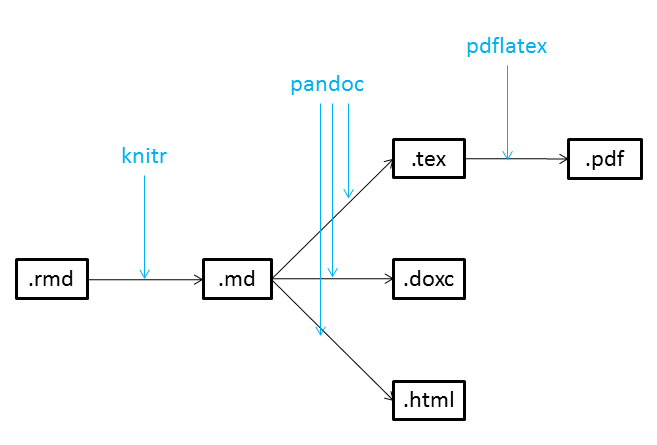
\includegraphics[width=5.20833in,height=\textheight]{../figures/pandoc1.png}

\begin{itemize}
\item
  If interested, follow this discussion:
  \href{https://ubuntuforums.org/showthread.php?t=395863}{\emph{Why
  LaTeX is such a bloated system?}}
\item
  So\ldots{}\href{https://yihui.name/tinytex/r/}{\emph{TinyTeX}} is a
  custom LaTeX distribution based on TeX Live that is small in size
  (\textasciitilde{}150MB) but functions well in most cases, especially
  for \texttt{R} users .
\item
  \texttt{tinytex} R package is a wrapper function that installs
  \emph{TinyTeX}.
\end{itemize}

\hypertarget{exercice-1-10min.}{%
\subsection{Exercice 1 (10min.)}\label{exercice-1-10min.}}

\begin{itemize}
\tightlist
\item
  Install the \texttt{tinytex} R package from the console. It may take a
  few minutes to download and compile (\textasciitilde{}150MB)
\end{itemize}

\begin{verbatim}
install.packages("tinytex")  
library(tinytex)  
install_tinytex()  
\end{verbatim}

\begin{itemize}
\item
  Create a new document, compile it as \emph{.pdf}.

  \begin{itemize}
  \tightlist
  \item
    Add a Table of Content.
  \item
    Add a graphic.
  \end{itemize}
\item
  Now compile it as a Word document (\emph{.docx})
\item
  Add some reference by specifying the \texttt{csl:\ ../csl/peerj.csl}
  and \texttt{bibliography:\ ../biblio/test\_library.bib} in the header
\end{itemize}

\hypertarget{latex-template}{%
\section{LaTeX template}\label{latex-template}}

\begin{itemize}
\item
  This allows further options in the \emph{.Rmd} file when going from
  \emph{.tex} file to \emph{.pdf}.
\item
  You can build your own \emph{.tex} template if you know LaTeX\ldots{}
\item
  There are many templates available on the web that you can use.
\item
  Here is one I like for
  \href{https://github.com/svmiller/svm-r-markdown-templates/blob/master/svm-latex-ms.tex}{manuscripts}
  (Thanks \href{https://github.com/svmiller}{svmiller} on
  
\includegraphics[width=0.3125in,height=\textheight]{../figures/octocat.png})

  \begin{itemize}
  \tightlist
  \item
    Using this (sligthly modified) template, I am writing
    \href{https://github.com/seb951/Acadian_seaplants/blob/master/manuscript_Rmd/Acadian_seaplants_v5.pdf}{my
    first \emph{.Rmd} manuscript}.\\
    \hspace*{0.333em}\\
    
\includegraphics[width=5.20833in,height=\textheight]{../figures/acadian.png}\\
    \hspace*{0.333em}\\
    \hspace*{0.333em}\\
  \end{itemize}
\item
  Here is one I like for
  \href{https://github.com/svmiller/svm-r-markdown-templates/blob/master/svm-latex-cv.tex}{\emph{Curriculum
  Vitae}}

  \begin{itemize}
  \tightlist
  \item
    Using this template, I re-wrote my
    \href{http://sebastien.renaut.com/wp-content/uploads/2019/02/cv.pdf}{CV}
    to give it a fresh look!\\
    \hspace*{0.333em}\\
    
\includegraphics[width=5.20833in,height=\textheight]{../figures/CV.png}
    ~\\
    \hspace*{0.333em}\\
  \end{itemize}
\item
  Download template and add it to the header. Not however that you
  should download or at least take a look at the
  \href{https://github.com/svmiller/svm-r-markdown-templates/blob/master/svm-rmarkdown-article-example.Rmd}{\emph{.Rmd}
  to see options}, and
  \href{https://github.com/svmiller/svm-r-markdown-templates/blob/master/svm-rmarkdown-article-example.pdf}{\emph{.pdf}
  to see output}.
\end{itemize}

\begin{Shaded}
\begin{Highlighting}[]
\NormalTok{--- }
\NormalTok{output:  }
\NormalTok{  pdf_document:  }
\NormalTok{   keep_tex: true  }
\NormalTok{   fig_caption: true  }
\NormalTok{   latex_engine: pdflatex  }
\NormalTok{   template: ../reference_material/svm-latex-ms.tex        }
\NormalTok{title: "**This is my first Rmarkdown manuscript**  }
\NormalTok{#many more options can go here which will be using by pdflatex.}
\NormalTok{---   }
\end{Highlighting}
\end{Shaded}

\begin{itemize}
\tightlist
\item
  You should know have all the tools to generate your fully reproducible
  manuscripts from \texttt{R}. The only objection I see is formatting
  manuscript this way is integrating comments from co-authors who do not
  use \texttt{R}, \texttt{R\ markdown}, \texttt{git} or \texttt{github}.
\end{itemize}

\hypertarget{exercice-2-10min.}{%
\section{Exercice 2 (10min.)}\label{exercice-2-10min.}}

\begin{itemize}
\item
  R packages \texttt{rticles} is (potentially) a nice package to format
  articles according to the specification of a journal.
\item
  But first, you need to install it in the R console.
\item
  Once installed, try starting a new R markdown document according to
  your journal of interest.
\end{itemize}

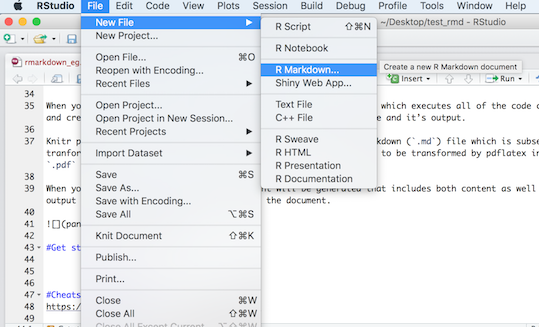
\includegraphics[width=5.20833in,height=\textheight]{../figures/getstarted.png}\\
\hspace*{0.333em}\\
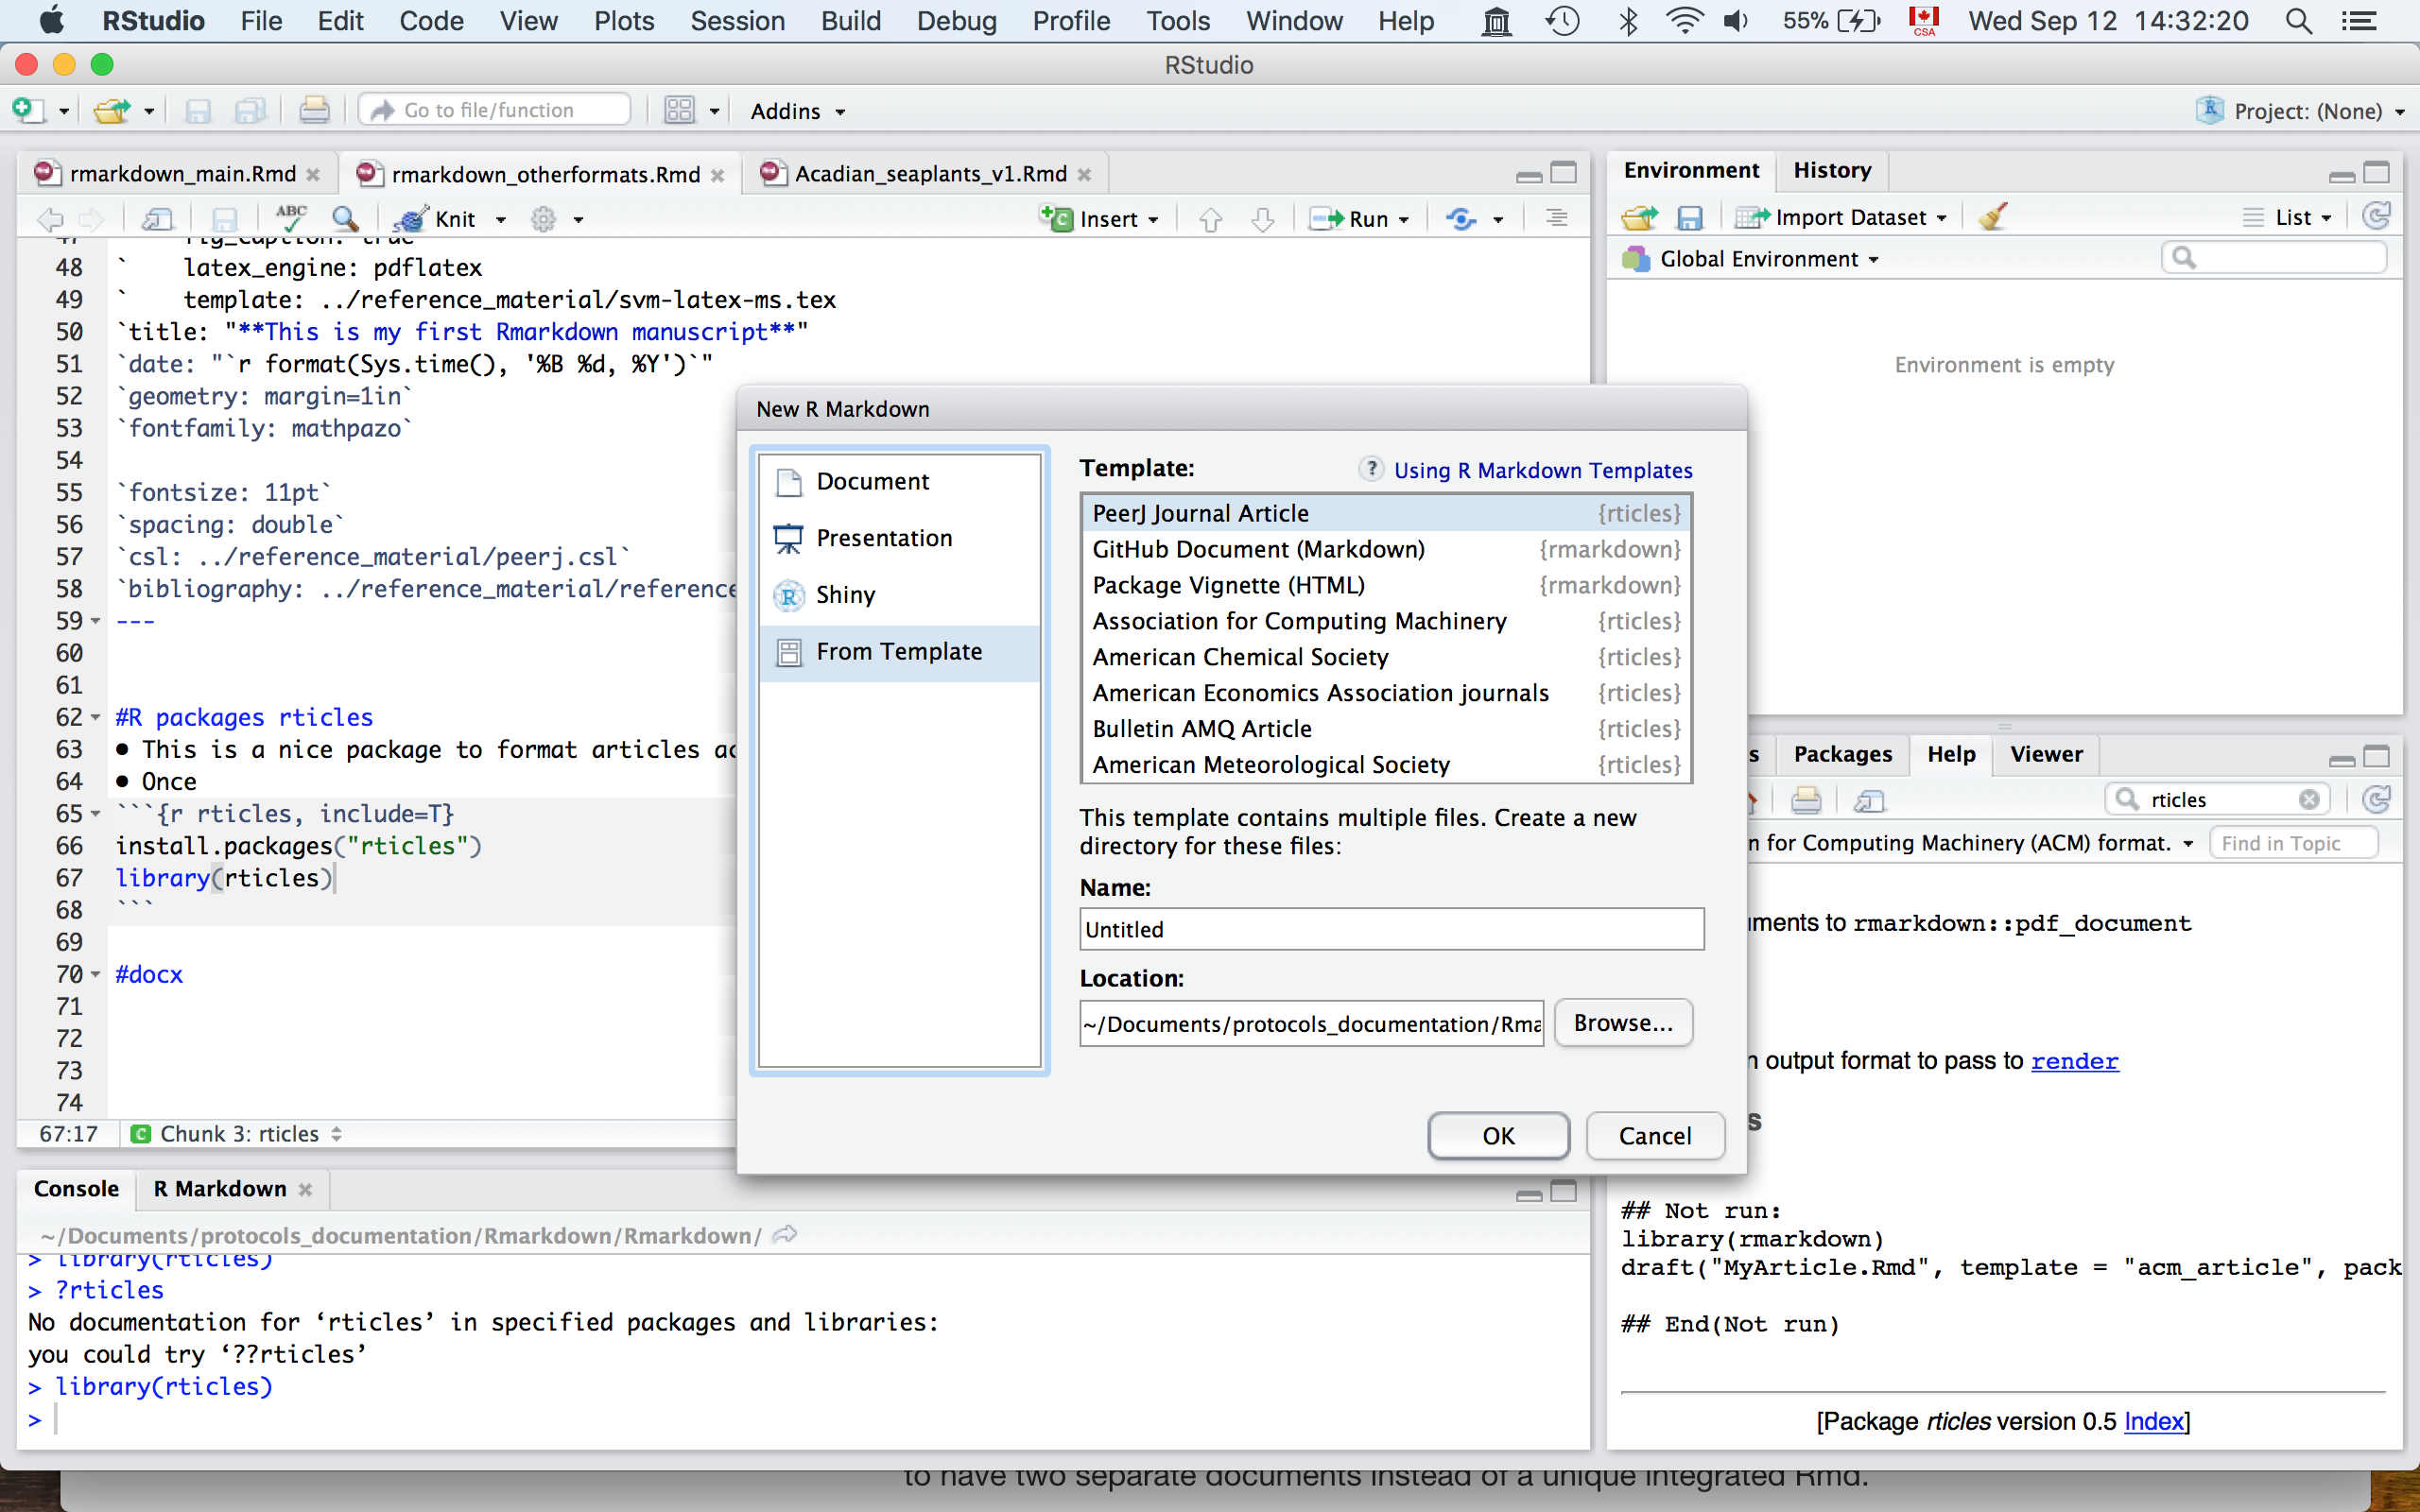
\includegraphics[width=5.20833in,height=\textheight]{../figures/from_template.png}\\
\hspace*{0.333em}

\begin{itemize}
\item
  Right now, few templates available.
\item
  Some templates may be slower to render, depending on what \emph{LaTeX}
  package they depend on and need to be downloaded (e.g PNAS).
\end{itemize}

\hypertarget{other-possibilities}{%
\section{Other possibilities}\label{other-possibilities}}

\hypertarget{presentations}{%
\subsection{Presentations}\label{presentations}}

\begin{itemize}
\tightlist
\item
  You can also generate Powerpoint-like presentations.\\
  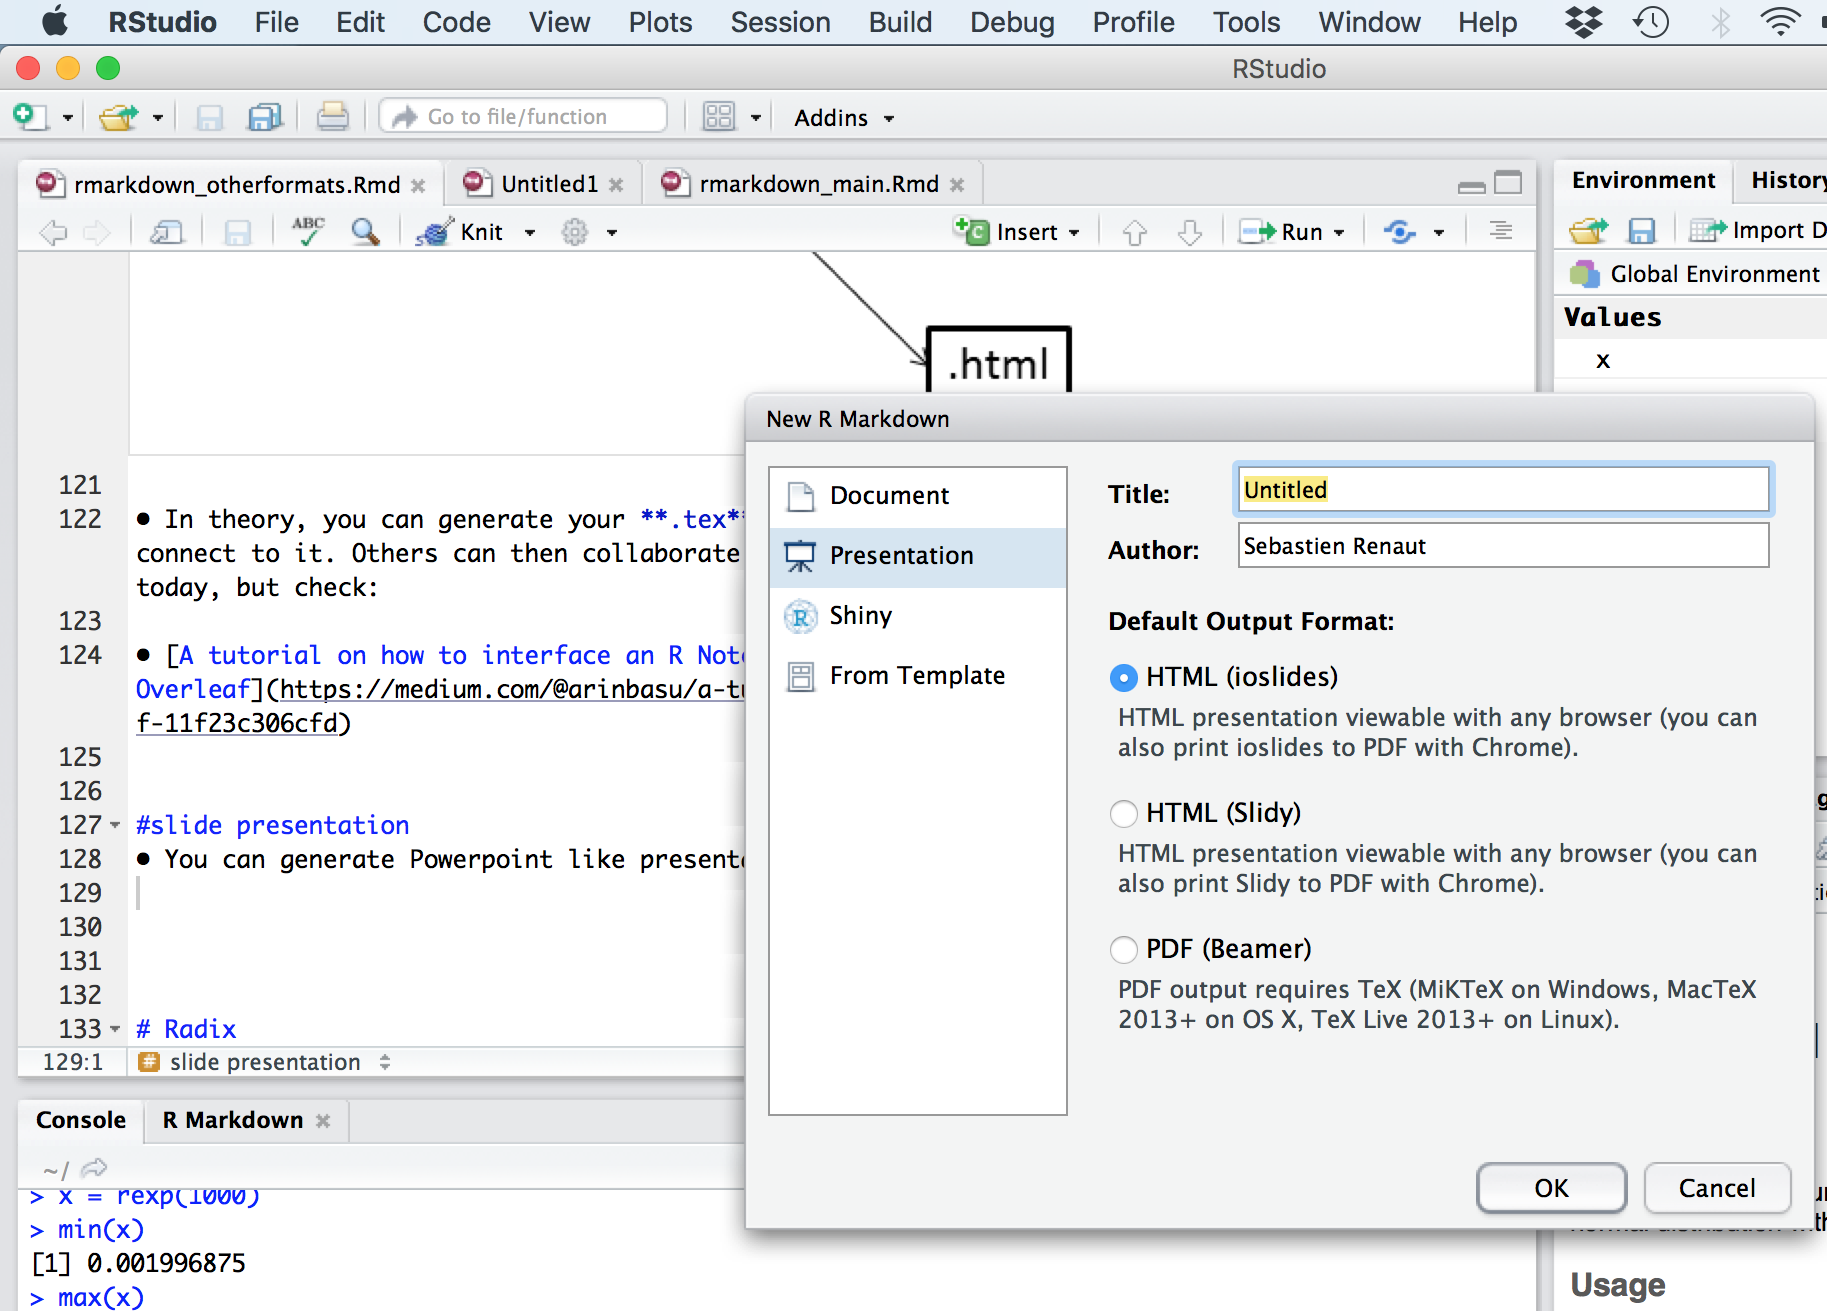
\includegraphics[width=4.16667in,height=\textheight]{../figures/slides.png}
\end{itemize}

\hypertarget{overleaf}{%
\subsection{Overleaf}\label{overleaf}}

\begin{itemize}
\tightlist
\item
  Overleaf is an online LaTeX and Rich Text collaborative writing and
  publishing tool that makes the whole process of writing, editing and
  publishing scientific documents much quicker and easier.
\end{itemize}

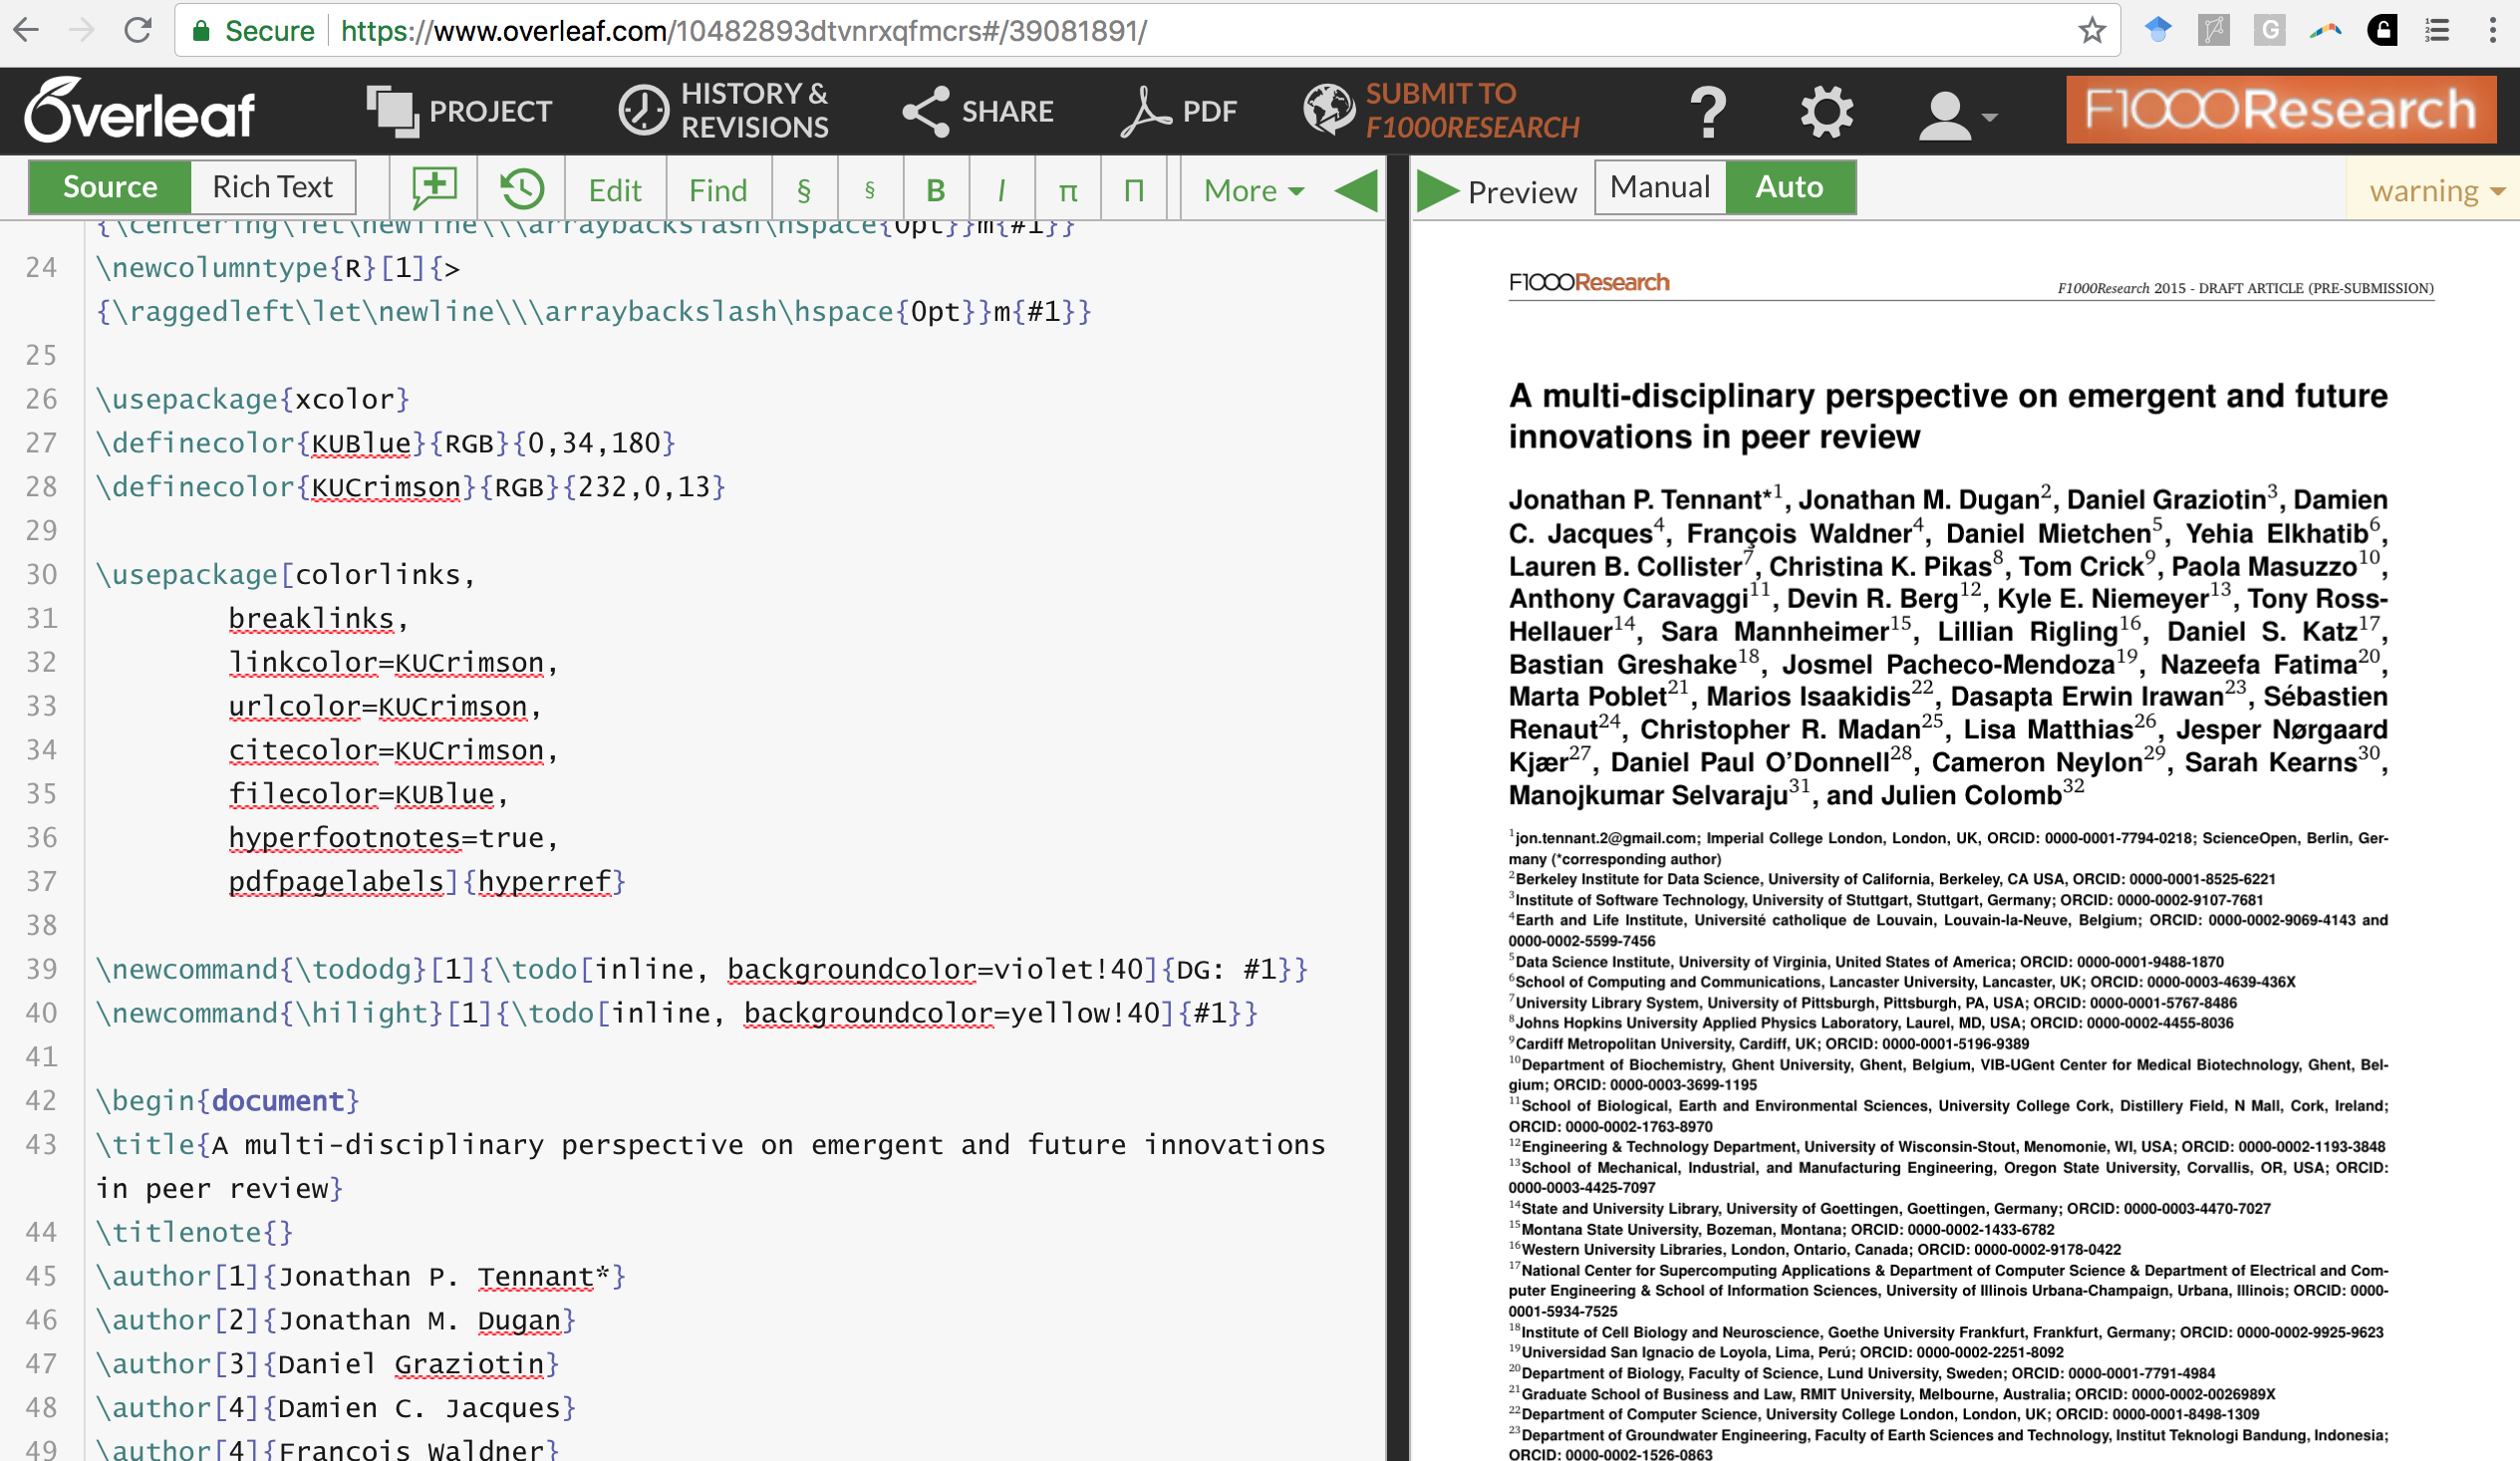
\includegraphics[width=5.20833in,height=\textheight]{../figures/overleaf.png}

\begin{itemize}
\item
  Remember this:\\
  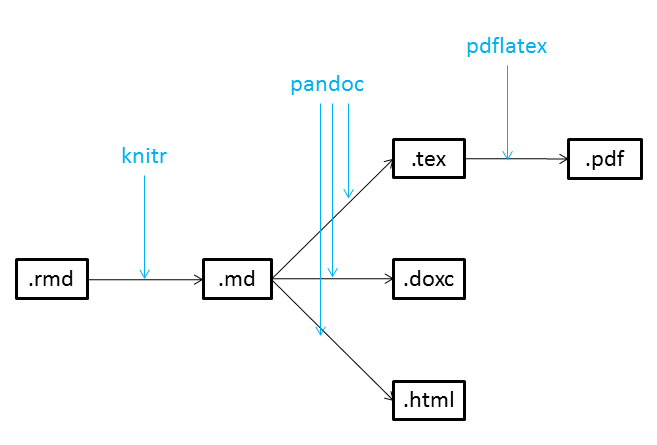
\includegraphics[width=5.20833in,height=\textheight]{../figures/pandoc1.png}
\item
  So you can generate your \emph{.tex} file, upload it to a github repo
  and Overleaf will connect to it. Others can then collaborate and
  modify the \emph{.tex} file.
\item
  Let's take a quick look at \href{https://www.overleaf.com/}{overleaf}.
  Once you have an overleaf account, you can connect it to a
  \href{https://www.github.com/}{github} repository. You can then
  pull/push from overleaf to github, allowing others to modify your
  \emph{.tex} file.
\end{itemize}

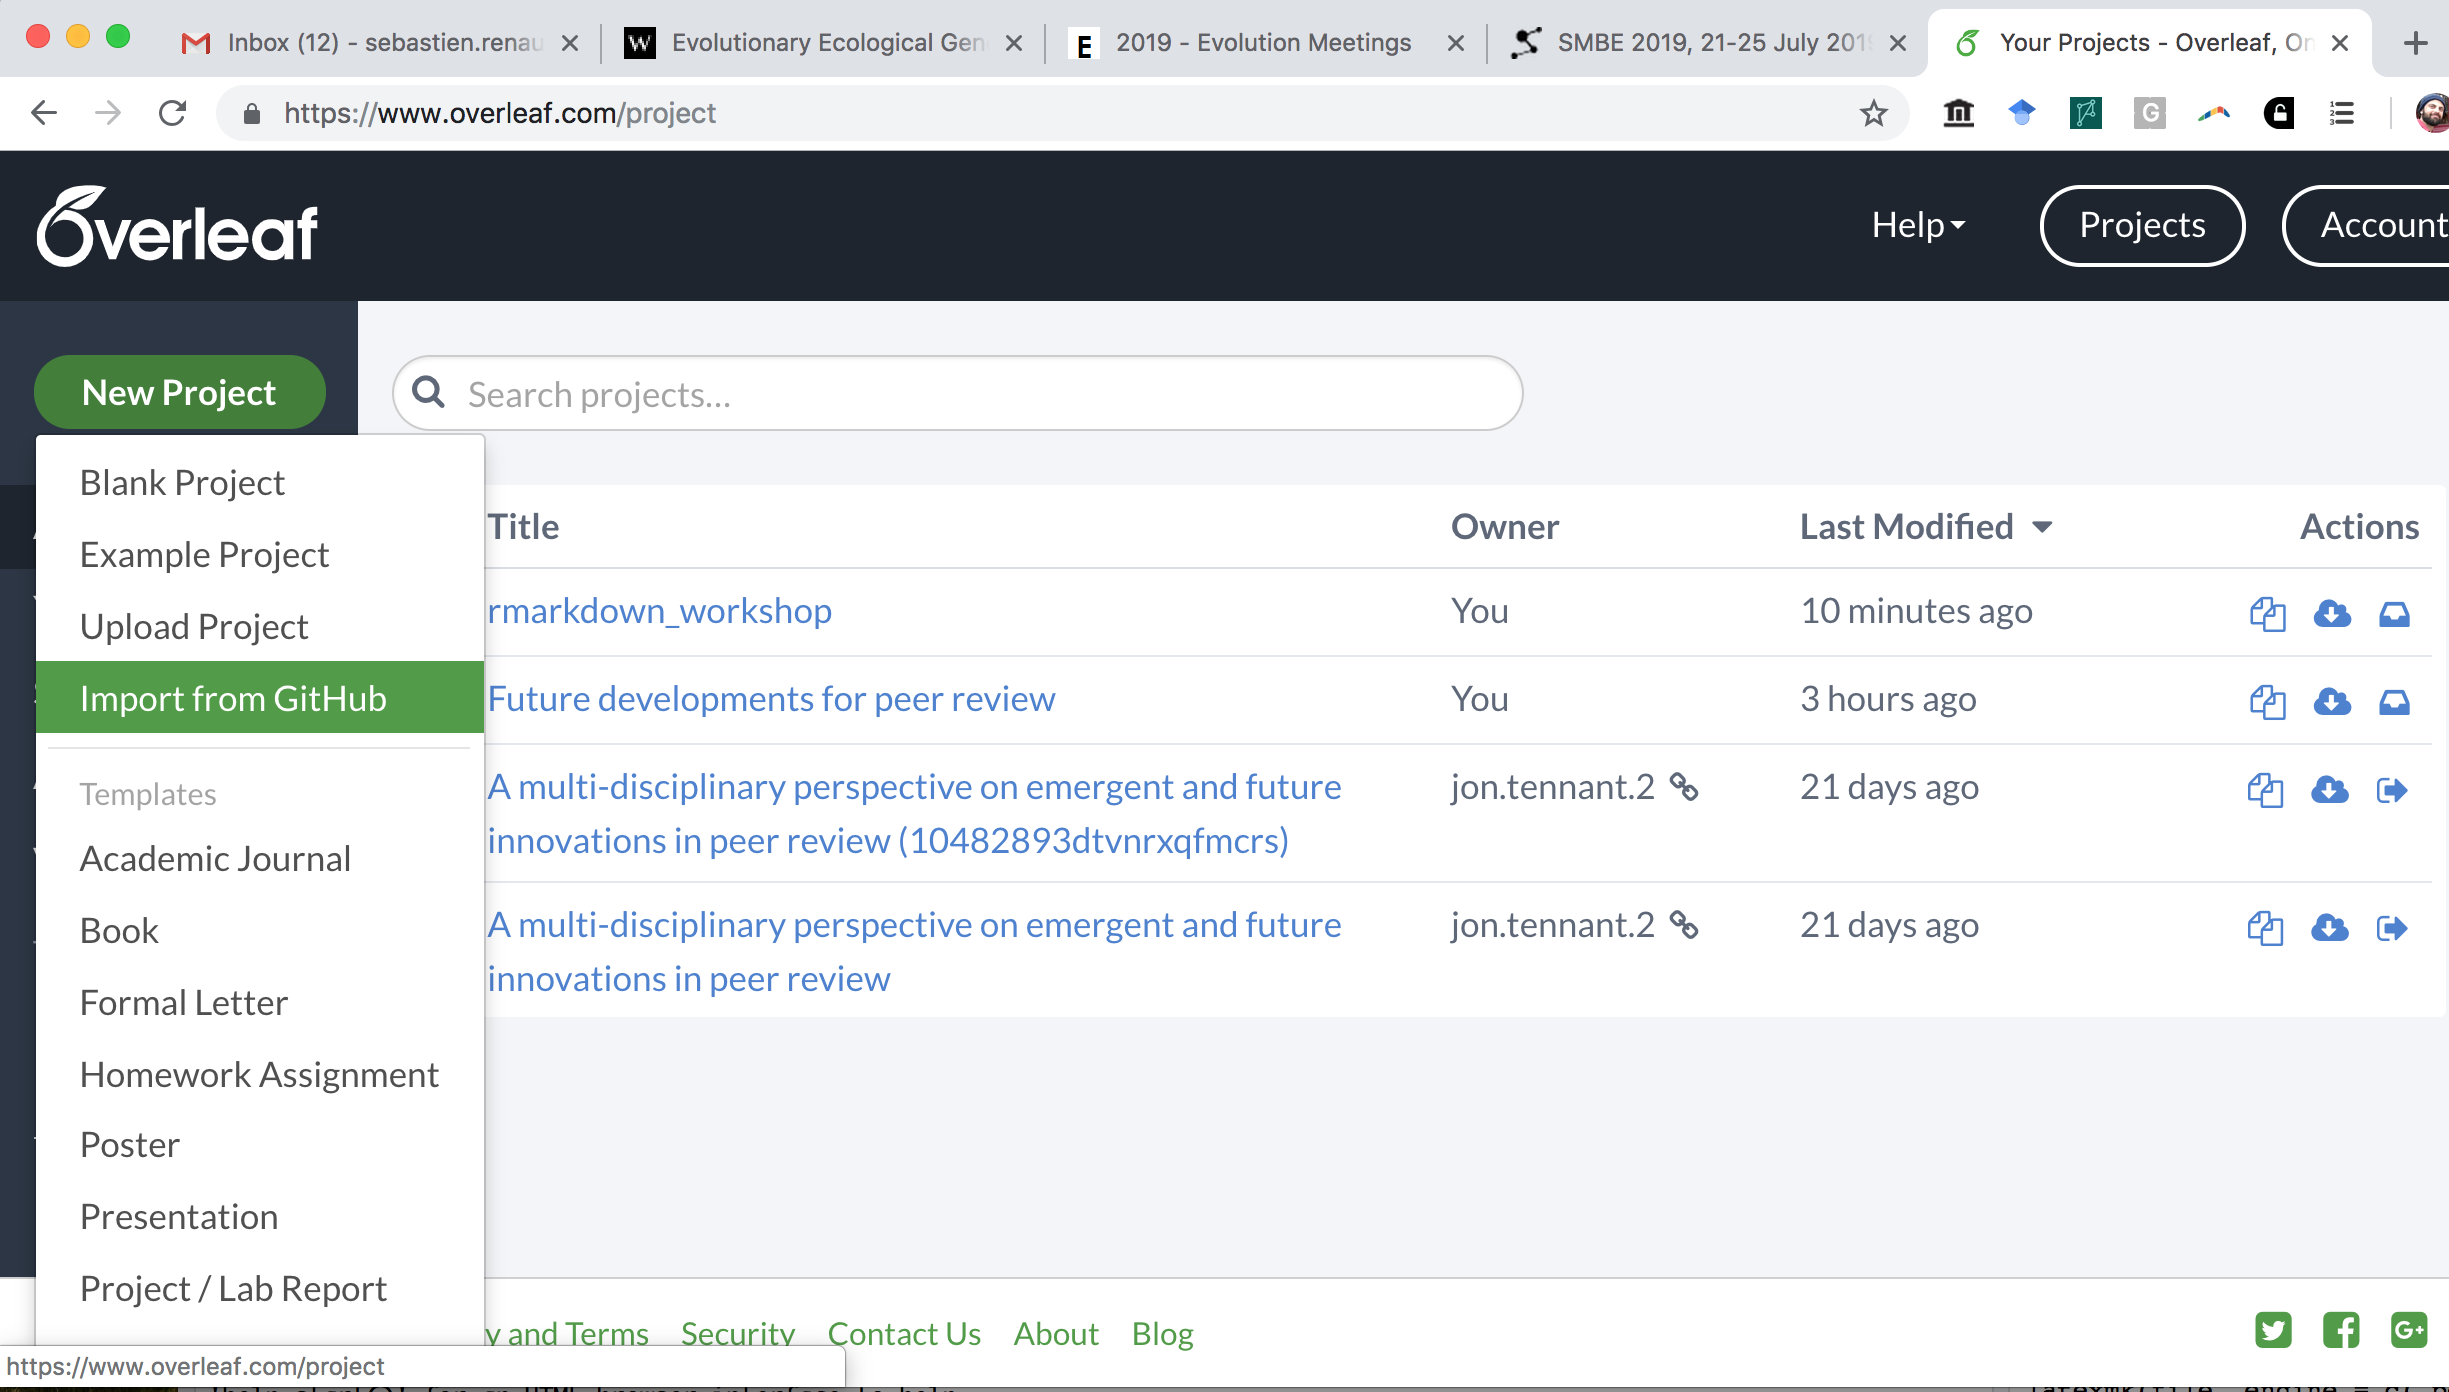
\includegraphics[width=5.20833in,height=\textheight]{../figures/overleaf_github.png}

\begin{itemize}
\item
  \href{https://medium.com/@arinbasu/a-tutorial-on-how-to-interface-an-r-notebook-with-overleaf-11f23c306cfd}{A
  tutorial on how to interface an R Notebook with Overleaf}
\item
  \href{https://www.overleaf.com/learn/how-to/How_do_I_connect_an_Overleaf_project_with_a_repo_on_GitHub,_GitLab_or_BitBucket\%3F}{How
  do I connect an Overleaf project with a repo on GitHub, GitLab or
  BitBucket?}
\end{itemize}

\hypertarget{bookdown}{%
\subsection{Bookdown}\label{bookdown}}

\begin{itemize}
\tightlist
\item
  \href{https://bookdown.org/}{Bookdown}
  
\includegraphics[width=0.20833in,height=\textheight]{../figures/bookdown.png}
  is an open-source R package that facilitates writing books and
  long-form articles/reports with R Markdown.
\end{itemize}


\includegraphics[width=5.20833in,height=\textheight]{../figures/rmarkdown.png}

\hypertarget{radix}{%
\subsection{Radix}\label{radix}}

\begin{itemize}
\item
  \href{https://blog.rstudio.com/2018/09/19/radix-for-r-markdown/}{Radix}
  offers a better look for publishing blog, webpages, adapted to mobile
  devices.\\
  
\includegraphics[width=5.20833in,height=\textheight]{../figures/radix.png}
\item
  You will need
  \href{https://www.rstudio.com/products/rstudio/download/preview/}{Rstudio
  v1.2}, \texttt{radix} and \texttt{leaflet}.
\end{itemize}

\begin{verbatim}
install.packages("radix")  
install.packages("leaflet")  
\end{verbatim}

\begin{itemize}
\tightlist
\item
  Change output in header to:
\end{itemize}

\begin{verbatim}
---  
title: "Rmarkdown: radix"  
author: "Sébastien Renaut"  
output: radix::radix_article  
---  
\end{verbatim}

\begin{itemize}
\tightlist
\item
  Then you can start playing with the \texttt{radix} options, such as in
  this example below (full width figures):
\end{itemize}

\begin{verbatim}
#Note that you may need to set eval = F for some formats (pdf, docx) to compile properly

```{r radix_example, echo = F, eval = T, layout='l-screen-inset'}  
library(leaflet)  
leaflet() %>%  
addTiles() %>%   
addMarkers(lng=174.768, lat=-36.852,popup="The birthplace of R")  
```    
\end{verbatim}

\hypertarget{exercice-3}{%
\subsection{Exercice 3}\label{exercice-3}}

\begin{itemize}
\item
  Use a previously generate document to generate a \texttt{radix} html
  output.
\item
  What does it look like? Better?
\end{itemize}

\begin{center}\rule{0.5\linewidth}{\linethickness}\end{center}


\end{document}
